\section{The optimization method}

The predefined parameters of a machine has drastic impact on the accuracy of the output. To get the best possible accuracy every possible combination of parameters would be need to be tested and compared, but such an approach becomes unfeasible very quickly. Even with only five parameters and the meager resolution of ten points per parameter, we would have to compute the RBM's prediction $10^5$ times. It would take a whole day even if each run is done within a second. To find a useable set of parameters we need to make some decisions of compromise to get within a practical time frame. We will heavily referee to Deep Learning \cite{Goodfellow}, written by Ian Goodfellow, Yoshua Begio and Aaron Courville, who has been in the forefront of the field. In chapter 11 and 12 they cover the best methods of approaching the problem at hand.

\vspace{\baselineskip}
For a overview of the approach we have chosen to use, we will give a shorten summary which is explained more in depth in each following section, together with the resulting parameters. To start of we want to find parameters that work best for each quantum system model and for every number of particles. The search time gets quickly out of control with greater system sizes, and as such we want to try to use regression to predict the best parameter for the upper end. As noted by Goodwill et. al. the hyperparameters is the most impactful so we will start by doing a search of optimal learning rate $\eta$. The number of hidden nodes is then searched, and for Gibbs sampling we will check the optimal number of sampling cycles.

\section{The Lipkin model}\label{sec:opt_lipkin}
\def \optgridwidhtratio {0.8}
\def \eat {\eta}
To determine the accuracy the RBM's output we will use the variance of the local energy, and not the error to the true solution. This may seem counter-intuitive, but by using the true ground state energy we will essentially slightly train the machine on data that it is not supposed to have. We have seen that for a machine state that matches a eigenstate of the Hamiltonian we get that:

$$Var[E_{local}] = 0 \;,$$

but this introduces another problem. The variance can approach zero even though it is not of an eigenstate of the Hamiltonian: if the state is dominated by a single basis-state. Therefore we will split off from all figures the parameters which causes the machine to fail to converge at all. Furthermore we will plot two variants of the variance, one of the variance of all the samples' local energy $Var[E(\boldsymbol{S})]$, and second the variance of the local energy of the basis states the machine state consists of, $Var[E(\boldsymbol{B})]$. Both are susceptible to skewed machine states, but on opposite ends. The first will drown out high differences between the basis state local energies by being dominated by a single state, while the other is very susceptible to just one copy of a wrong basis state in the samples. We will therefor choose variables of the quantum system where we expect a distribution of all basis states. But if the machine might still find a state with zero variance by mistake as seen here:

\def \impJ {2}
\def \impeps {1.5 - \frac{\sqrt{3}}{2}}
\def \impV {-1}
\def \impW {0}
\def \impk {1}

\begin{figure}[H]
  \begin{center}
    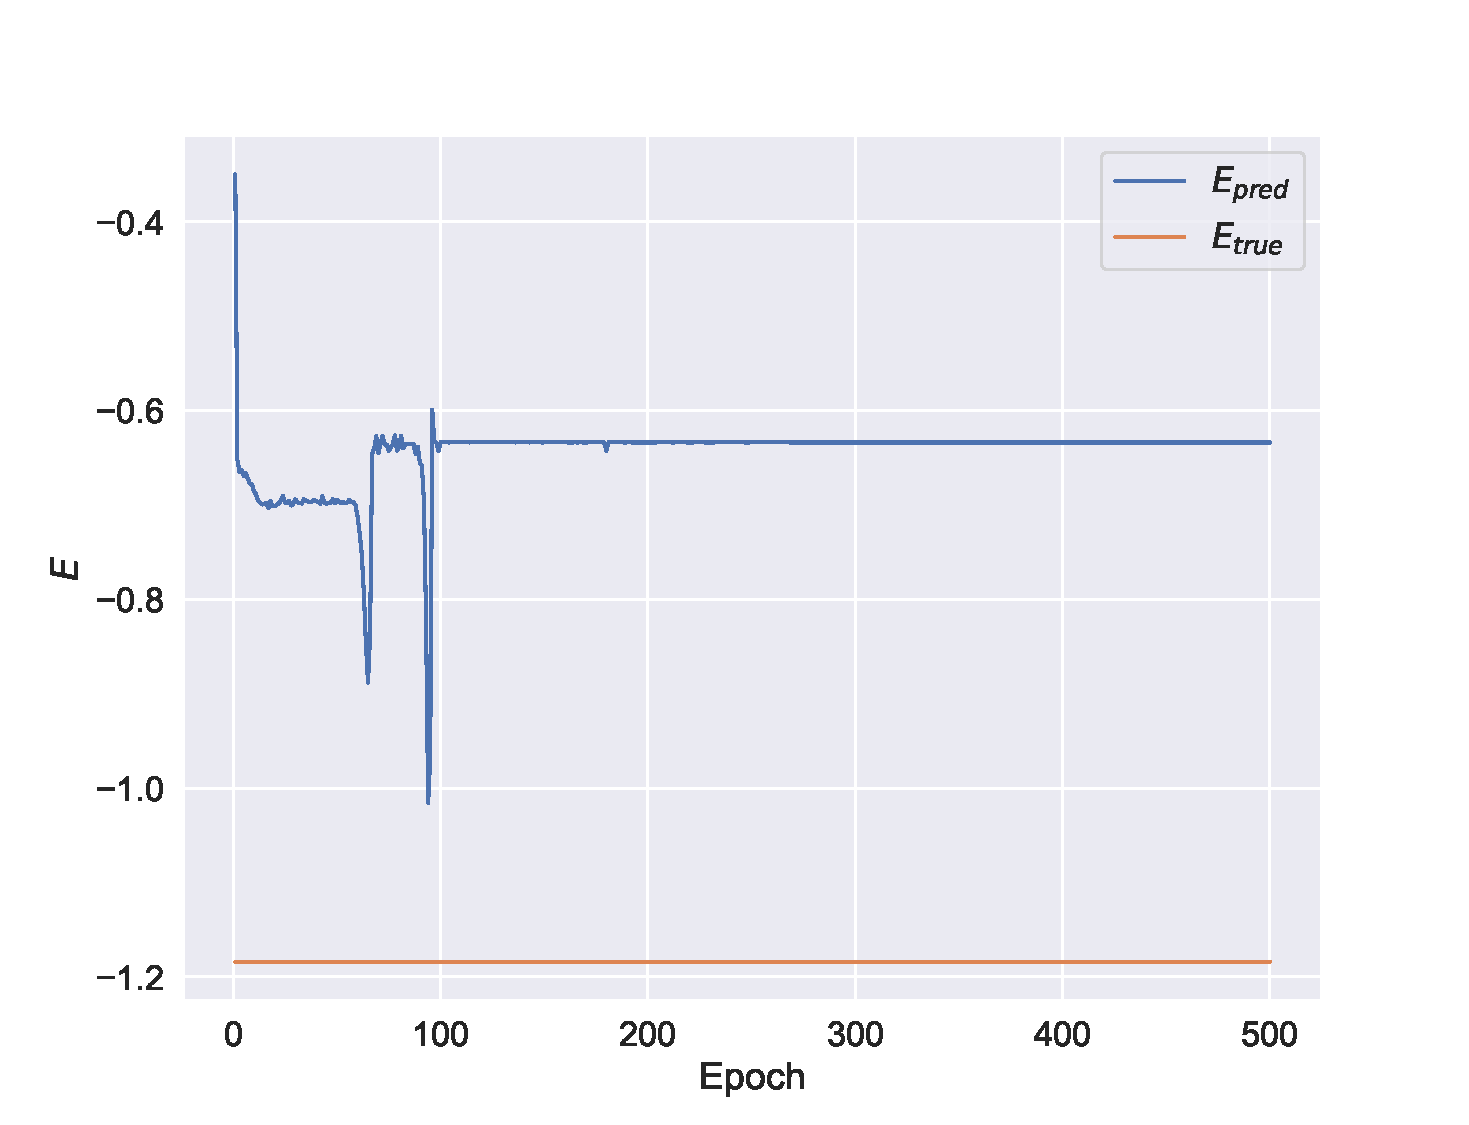
\includegraphics[width=0.95\textwidth]{Figures/Plots/OPt/wrong_state.pdf}
  \end{center}
  \caption{The machine in the wrong state, but still achieving close to zero variance of the local energy of each sample. Here the $J = \impJ$ Lipkin model is used with $\varepsilon = \impeps$, $V = \impV$ and $W = \impW$. The number of hidden nodes has here been increased to $20$ and the learning rate is at $\eta = 3$.}\label{fig:wrong_state}
\end{figure}

We will therefore watch the variance of the local energy of the basis states as well, which will increase when the machine state is wrongly dominated by a single basis state. To begin we set up the resulting array first.

\begin{minted}{python}
resolution = 10
samples_var = np.zeros(resolution)
basis_var = np.zeros(resolution)
\end{minted}

and we iterate through the two axes:

\begin{minted}{python}
for i in range(resolution):
    for j in range(resolution):
        
        run_options['adaptive_function'] = adaptives.nop
        run_options['learning_rate'] = search_y[i]

        result = main.run(
            model_options,
            machine_options,
            run_options,
            "",
            log = False,
            verbose = verbose
        )
        
        samples_var[i] = result['variance'][-1]
        basis_var[i] = result['part_var'][-1]
\end{minted}

First we attempt to find a suitable range of learning rates to look closer at. Starting of with a wide range of learning rates, $\eta =1 \rightarrow \eta = 12$, so that we can zoom in on the lower parts afterwards instead.  We use $50$ data points, but to make sure there are no random outlier we will take the average over five repetitions. We use the Lipkin model with $2$ particles and the other parameters and model options are:

\begin{itemize}
  \item Monte Carlo cycles (number of samples) : $50 000$
  \item Epochs : $500$
  \item Number of hidden nodes : $4$
  \item $\varepsilon = \impeps$
  \item $V = \impV$
  \item $W = \impW$
\end{itemize}

We then get:

\begin{figure}[H]
  \begin{center}
    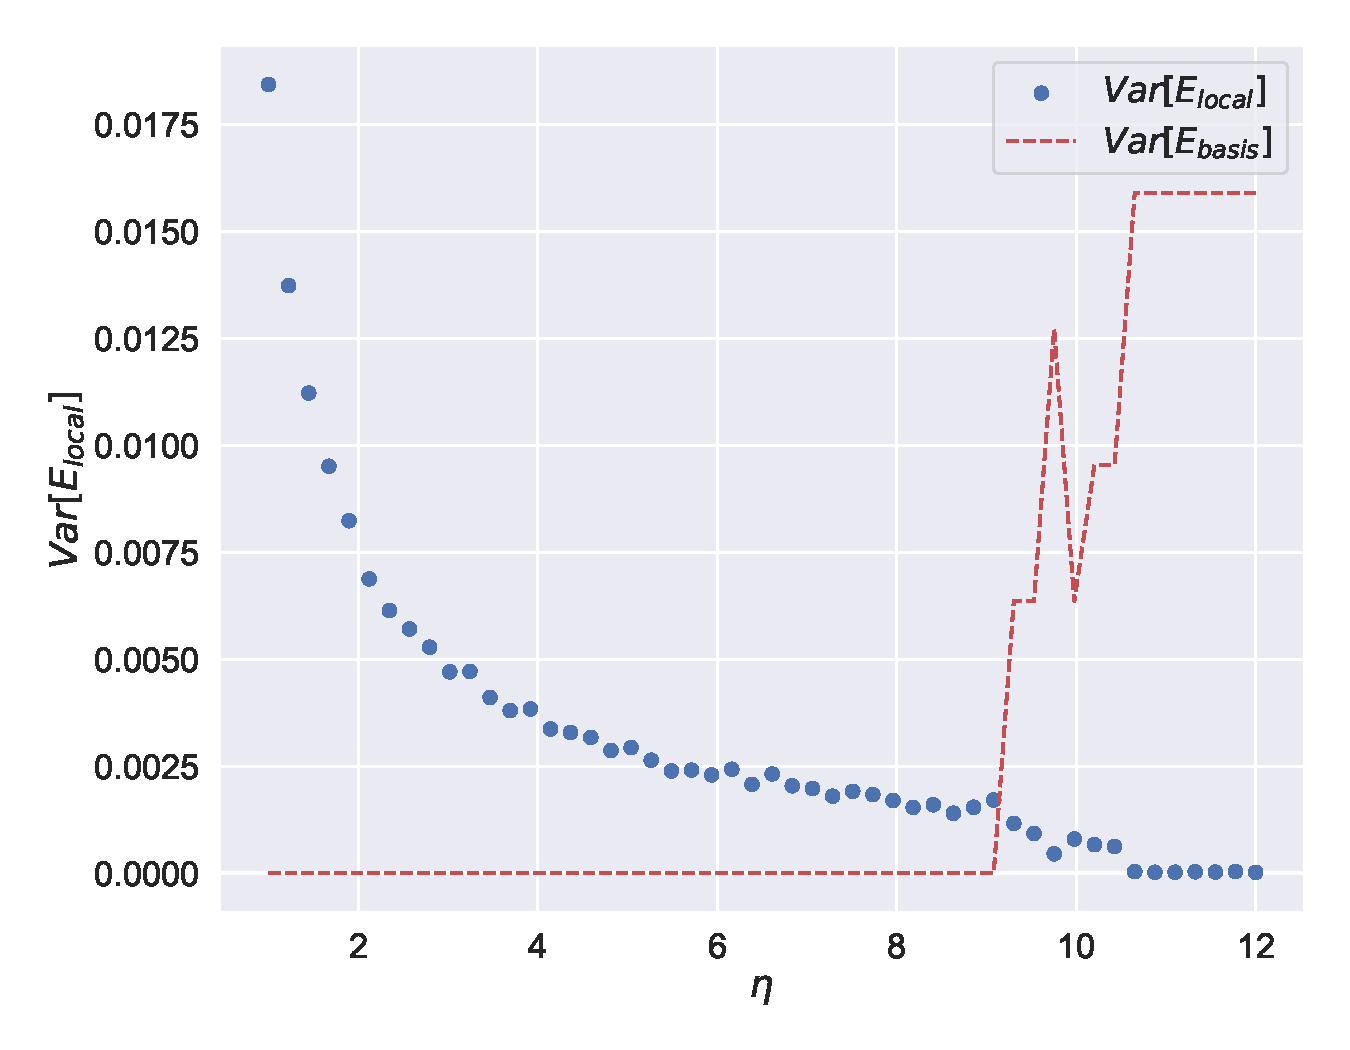
\includegraphics[width=\optgridwidhtratio\textwidth]{Figures/Plots/OPt/Lipkin/[2][learning_rate][e=500][1.0-12.0]}
  \end{center}
  \caption{First search of optimal learning rate $\eta$. The variance of the local energy of each sample together with the variance of the local energy of each basis state. The variance of $E_{basis}$ has been normalized to stay in the same range as $E_{local}$ to make it readable. The Lipkin model is used with $\varepsilon = \impeps$, $V = \impV$ and $W = \impW$.}\label{fig:lr_depth1}
\end{figure}

The value of $Var[E_{basis}]$ is not that important, but it is rather the increase and decrease we are interested in, so we have normalized the array to match the same range of values as that of $Var[E_{local}]$. In \ref{fig:lr_depth1} the variance decreases smoothly towards around $\eta = 9$ to $\eta = 10$ where it dips down suddenly. At this point the variance of the basis state's local energy spikes up, indicating that the machine defaulted back to a single basis state wavefunction. We look closer at the range $\eta = 7 \rightarrow \eta = 9$, and we get:

\begin{figure}[H]
  \begin{center}
    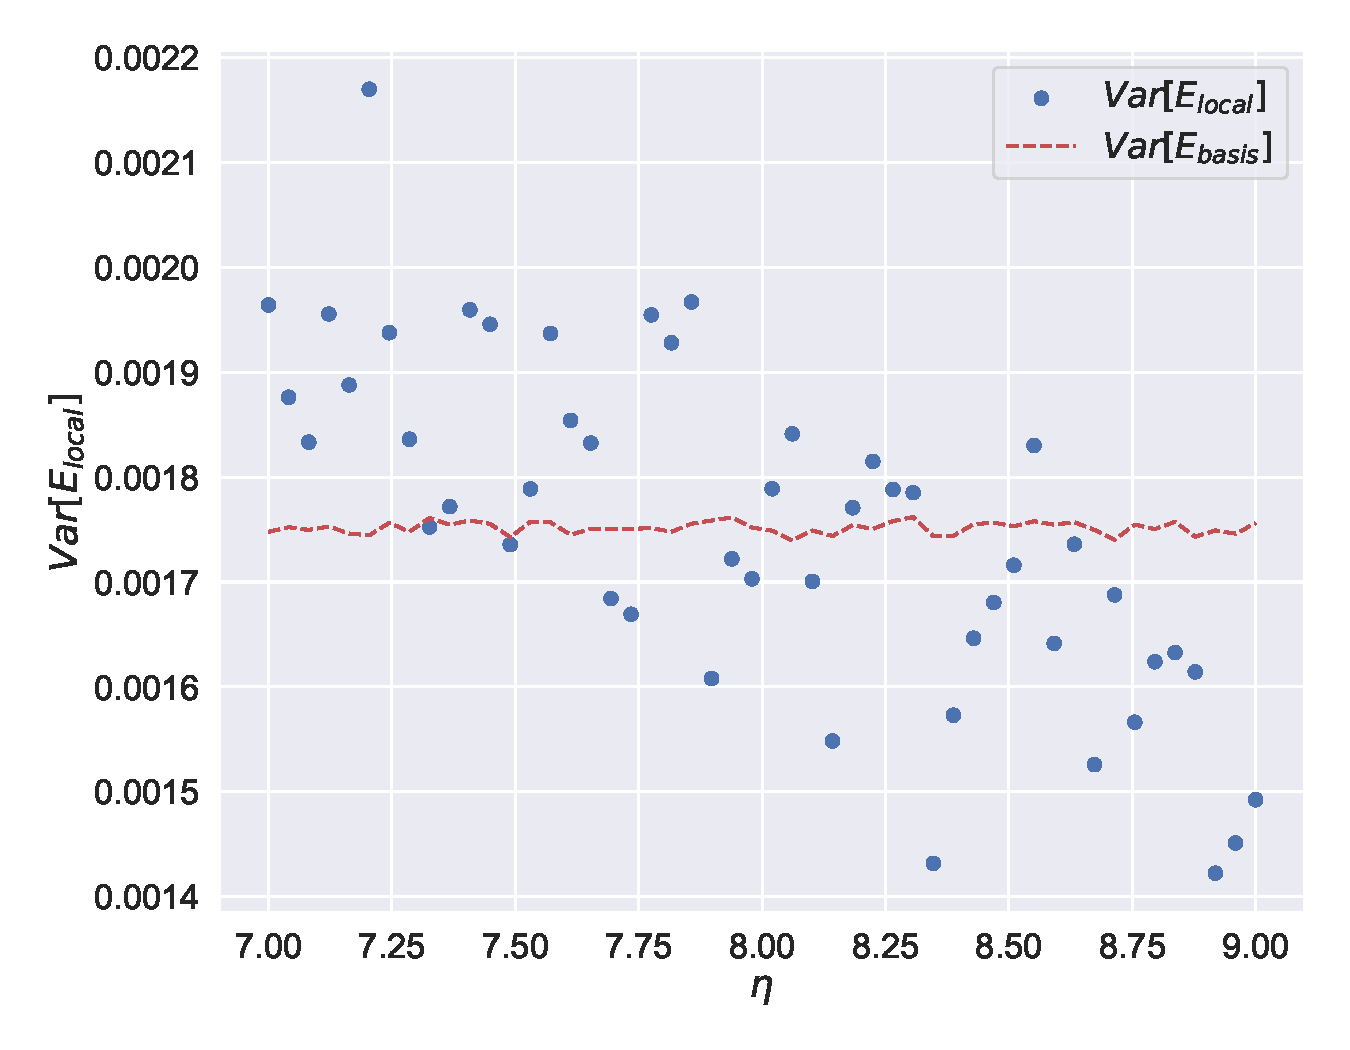
\includegraphics[width=\optgridwidhtratio\textwidth]{Figures/Plots/OPt/Lipkin/[2][learning_rate][e=500][7.0-9.0]}
  \end{center}
  \caption{The variance of the local energy of each sample together with the variance of the local energy of each basis state. The variance of $E_{basis}$ has been normalized to stay in the same range as $E_{local}$ to make it readable. The Lipkin model is used with $\varepsilon = \impeps$, $V = \impV$ and $W = \impW$.}\label{fig:lipkin_opt_ng_depth2}
\end{figure}

$Var[E_{local}]$ is now a bit more unstable, but it is possible to distinguish a downwards trend towards $\eta = 9$. We will then stop the search here, and since $Var[E_{basis}]$ stays consistent we choose the lowest $Var[E_{local}]$, which is at $\eta = 8.92$. Next step is then to check what number of hidden nodes gives the best accuracy, and we now set the learning rate to the one we just determined to be optimal. For $h_n = 2 \rightarrow h_n = 11$ we get the following:

\begin{figure}[H]
  \begin{center}
    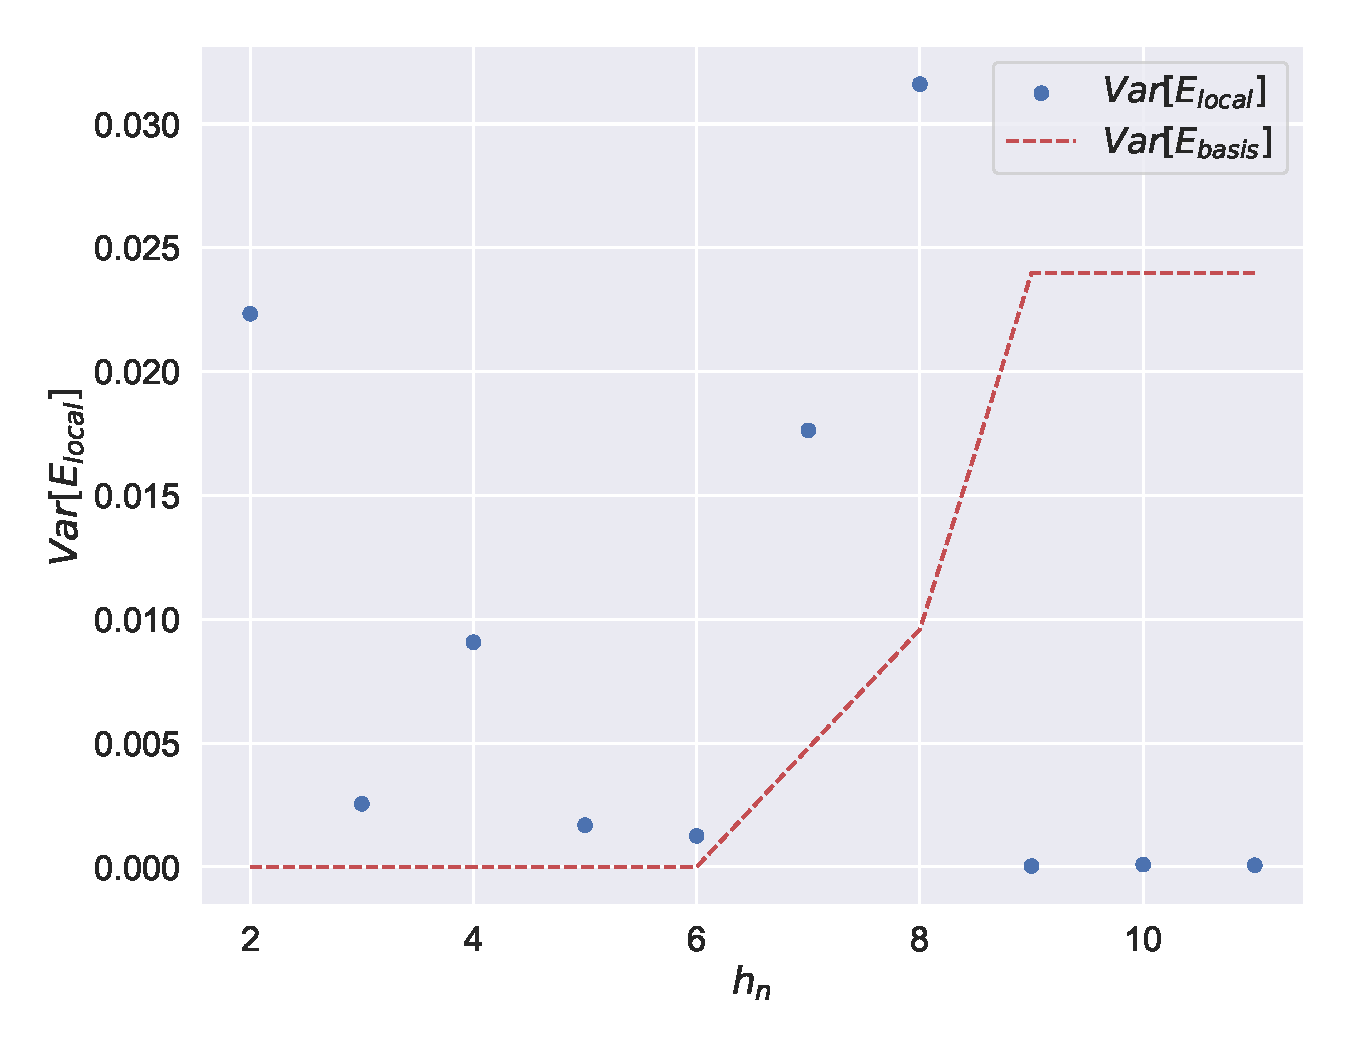
\includegraphics[width=\optgridwidhtratio\textwidth]{Figures/Plots/OPt/Lipkin/[2][hidden_n][e=500][2-11].pdf}
  \end{center}
  \caption{Search for optimal number of hidden nodes when $\eta = 8.92$. In the plot is the variance of the local energy of each sample together with the variance of the local energy of each basis state. The variance of $E_{basis}$ has been normalized to stay in the same range as $E_{local}$ to make it readable. The Lipkin model is used with $\varepsilon = \impeps$, $V = \impV$ and $W = \impW$.}\label{fig:hn_depth1}
\end{figure}

It is clear that after $h_n = 6$ the machine struggles to find the correct wavefunction. For hidden nodes we can't look any closer than integer values, so we choose the lowest variance again, this time at $h_n = 6$. We then do the same thing for the number of Gibbs sampling cycles, with $k = 1 \rightarrow k=10$,
\begin{figure}[H]
  \begin{center}
    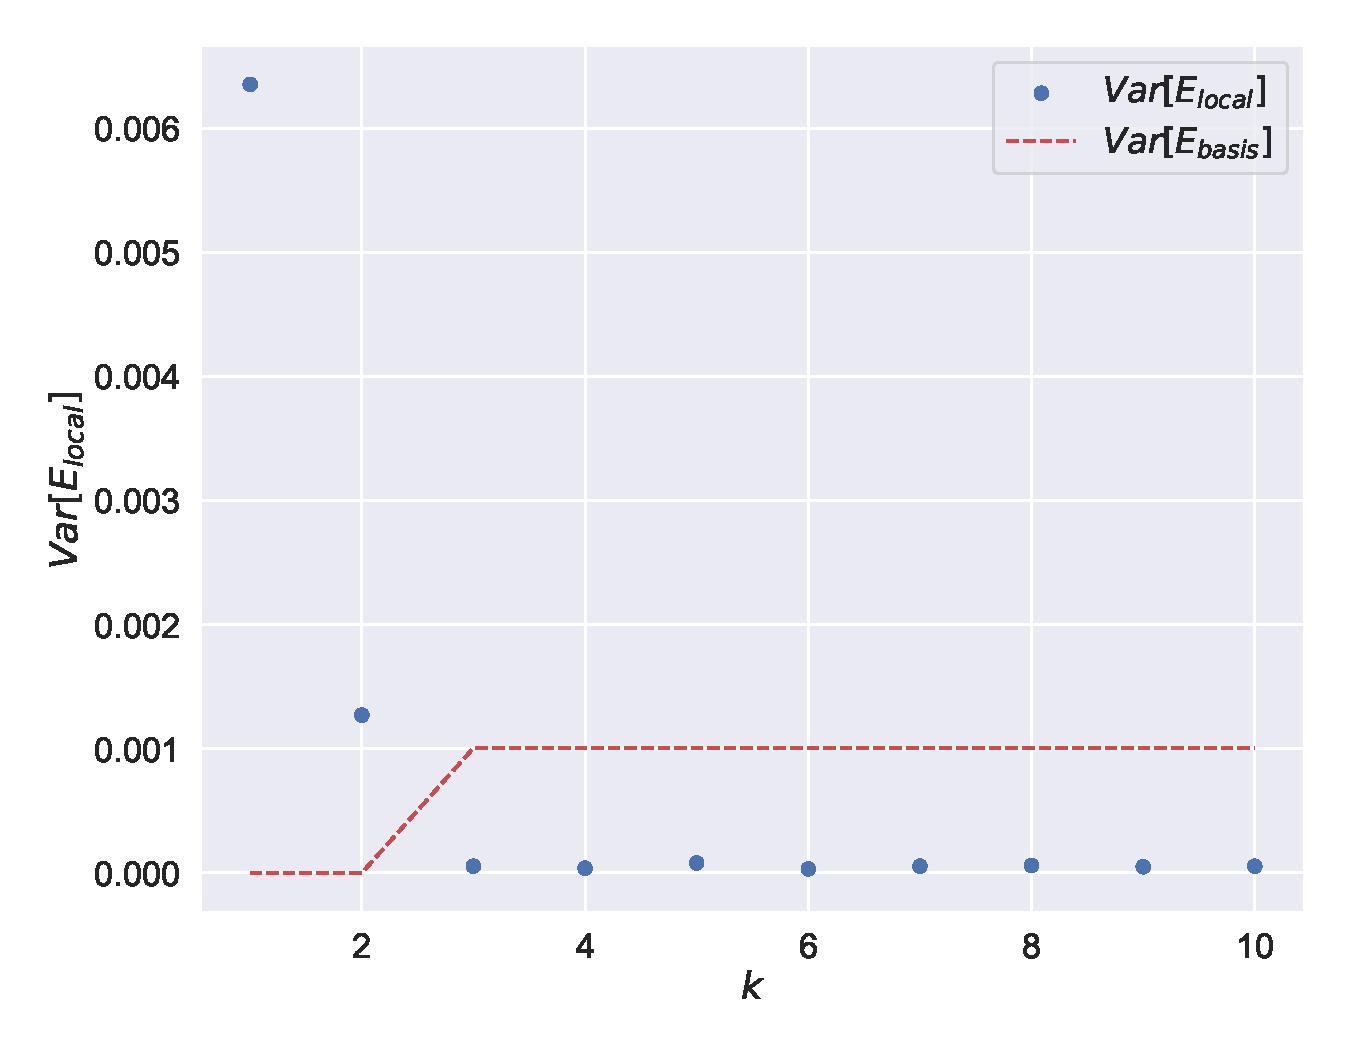
\includegraphics[width=\optgridwidhtratio\textwidth]{Figures/Plots/OPt/Lipkin/[2][gibbs_k][e=500][1-10].pdf}
  \end{center}
  \caption{Search for optimal number of Gibbs sampling cycles when $\eta = 8.92$. In the plot is the variance of the local energy of each sample together with the variance of the local energy of each basis state. The variance of $E_{basis}$ has been normalized to stay in the same range as $E_{local}$ to make it readable. The Lipkin model is used with $\varepsilon = \impeps$, $V = \impV$ and $W = \impW$.}\label{fig:hn_depth2}
\end{figure}

We see a clear dip in $Var[E_{local}]$ from $k =1$ to $k=2$, and right after that the $Var[E_{basis}]$ jumps up, so we set $k=2$ to be optimal for the Lipkin model at $2$ particles.

\subsection{Predicting optimal parameters}

For the learning rate $\eta$, the number of hidden nodes, and the number of cyces $k$ we want to predict the optimal value as the system size increases. We will use regression and try to fit our data found by hand to a function $f_p(n)$ of parameter $p$ that takes in the size of the system. We will try two different types of ansatz for the learning rate parameter:

\vspace{\baselineskip}

Exponential decrease:

\begin{equation}
  f_p(n) = a e^{-b*n} + c
  \label{eq:fit_function}
\end{equation}

\vspace{\baselineskip}


Rational decrease:

\begin{equation}
  f_p(n) = \frac{a}{(x+b)} + c
  \label{eq:ratioanl_decrease}
\end{equation}

These two we think is most likely to fit the optimal learning rate data best, but for $h_n$ and $k$ we want to for linear increase:

\begin{equation}
  f_p(n) = ax + b
  \label{eq:linear_increase}
\end{equation}

We use the SciPy\cite{2020SciPy-NMeth} python library to fit our data to the curve with the \mintinline{python}{curve_fit} method:

\begin{minted}{python}
def inverse(x, a, b, c):
    return a/(x+b) + c

def exponential(x, a, b, c):
    return a*np.exp(-b*x) + c

abc = np.array([1, 1, 1])
fitted_inv, pcov_inv    = curve_fit(inverse, x, y, abc)
fitted_exp, pcov_exp    = curve_fit(exponential, x, y, abc)
\end{minted}

And we choose the one with least variance in the fitted result. With this we get for the Lipkin model that the exponential decrease is the best fit for learning rate:

\begin{figure}[H]
  \begin{center}
    \includegraphics[width=0.95\textwidth]{}
  \end{center}
  \caption{The fitted curve or the learning rate for the Lipkin model ground state energy predictions. The curve type here is exponential decrease, \ref{eq:fit_function}.}\label{fig:lipkin_imp_fit_lr}
\end{figure}

And for $\gamma$ we get:

\begin{figure}[H]
  \begin{center}
    \includegraphics[width=0.95\textwidth]{}
  \end{center}
  \caption{The fitted curve or the $\gamma$ momentum parameter for the Lipkin model ground state energy predictions. The curve type here is exponential decrease, \ref{eq:fit_function}.}\label{fig:lipkin_imp_fit_gamma}
\end{figure}

We can then summarize the parameters in a table.

\subsection{Final parameters}
\begin{table}[H]
  \caption{The final parameters chosen for the Lipkin model for different sizes. The colored boxes are derived from regression of the calculated data points.}\label{tab:lipkin_parameters}
  \begin{center}
    \begin{tabular}{|l|l|l|l|l|l|l|l|l|l|}
      \hline
      \textbf{size} & $2$ &$3$ & $4$& $5$& $6$& $7$&$8$ &$9$ & $10$ \\
      \hline
      $\eta$ & & & & & & & & & \\
      \hline
      $\gamma$ & & & & & & & & &  \\ 
      \hline
      $h_n$ & & & & & & & & & \\
      \hline
      \hline
      \textbf{size} & $2$ &$3$ & $4$& $5$& $6$& $7$&$8$ &$9$ & $10$ \\
      \hline
      $\eta$ & & & & & & & & &   \\
      \hline
      $\gamma$ & & & & & & & & &   \\ 
      \hline
      $h_n$ & & & & & & & & &  \\
      \hline

    \end{tabular}
  \end{center}
\end{table}


\section{The Ising model}
\begin{table}[H]
  \caption{The final parameters chosen for the Ising model for different sizes. The colored boxes are derived from regression of the calculated data points.}\label{tab:Ising_parameters}
  \begin{center}
    \begin{tabular}{|l|l|l|l|l|l|l|l|l|l|}
      \hline
      \textbf{size} & $2$ &$3$ & $4$& $5$& $6$& $7$&$8$ &$9$ & $10$ \\
      \hline
      $\eta$ & & & & & & & & & \\
      \hline
      $\gamma$ & & & & & & & & &  \\ 
      \hline
      $h_n$ & & & & & & & & & \\
      \hline
      \hline
      \textbf{size} & $2$ &$3$ & $4$& $5$& $6$& $7$&$8$ &$9$ & $10$ \\
      \hline
      $\eta$ & & & & & & & & &   \\
      \hline
      $\gamma$ & & & & & & & & &   \\ 
      \hline
      $h_n$ & & & & & & & & &  \\
      \hline

    \end{tabular}
  \end{center}
\end{table}


\section{The Heisenberg model}
\begin{table}[H]
  \caption{The final parameters chosen for the Heisenberg model for different sizes. The colored boxes are derived from regression of the calculated data points.}\label{tab:Heisenberg_parameters}
  \begin{center}
    \begin{tabular}{|l|l|l|l|l|l|l|l|l|l|}
      \hline
      \textbf{size} & $2$ &$3$ & $4$& $5$& $6$& $7$&$8$ &$9$ & $10$ \\
      \hline
      $\eta$ & & & & & & & & & \\
      \hline
      $\gamma$ & & & & & & & & &  \\ 
      \hline
      $h_n$ & & & & & & & & & \\
      \hline
      \hline
      \textbf{size} & $2$ &$3$ & $4$& $5$& $6$& $7$&$8$ &$9$ & $10$ \\
      \hline
      $\eta$ & & & & & & & & &   \\
      \hline
      $\gamma$ & & & & & & & & &   \\ 
      \hline
      $h_n$ & & & & & & & & &  \\
      \hline

    \end{tabular}
  \end{center}
\end{table}


\section{The Pairing model}
\begin{table}[H]
  \caption{The final parameters chosen for the Pairing model for different sizes. The colored boxes are derived from regression of the calculated data points.}\label{tab:Pairing_parameters}
  \begin{center}
    \begin{tabular}{|l|l|l|l|l|l|l|l|l|l|}
      \hline
      \textbf{size} & $2$ &$3$ & $4$& $5$& $6$& $7$&$8$ &$9$ & $10$ \\
      \hline
      $\eta$ & & & & & & & & & \\
      \hline
      $\gamma$ & & & & & & & & &  \\ 
      \hline
      $h_n$ & & & & & & & & & \\
      \hline
      \hline
      \textbf{size} & $2$ &$3$ & $4$& $5$& $6$& $7$&$8$ &$9$ & $10$ \\
      \hline
      $\eta$ & & & & & & & & &   \\
      \hline
      $\gamma$ & & & & & & & & &   \\ 
      \hline
      $h_n$ & & & & & & & & &  \\
      \hline

    \end{tabular}
  \end{center}
\end{table}

